\section{Wellen}

\subsection{Definition}

Eine Welle ist eine \textbf{Störung} eines \textbf{Gleichgewichtszustands}, die sich \textbf{im Raum ausbreitet}.


\subsubsection{Bemerkungen zur Definition}

\begin{outline}
    \1 Voraussetzung für \textbf{Ausbreitung} einer Welle ist \textbf{Kopplung} benachbarter Teilchen
    \1 Störung kann von ganz unterschiedlicher Natur sein: 
        \2 Druck in Luft
		\2 Auslenkung einer Position entlang einem Seil (Saite)
		\2 Eletrische Signale  
\end{outline}

\smallskip

\textbf{ \textrightarrow\ Die Störung wird mit $\bm{\xi}$ beschrieben:} $\bm{\xi = \xi(x, y, z, t)}$ 



\subsection{Klassifizierung von Wellen}

\begin{minipage}[t]{0.5\columnwidth}
    \paragraph{Transversalwellen}

    Welle breitet sich \textbf{senkrecht} zur Störung aus

    \begin{center}
        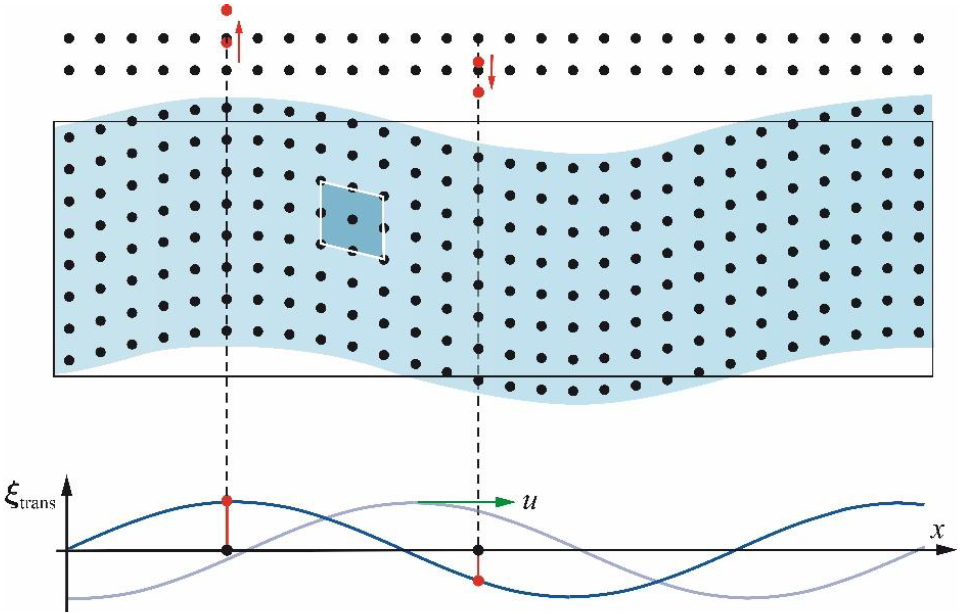
\includegraphics[height=2.6cm, align=t]{images/welle_transversal.png}
    \end{center}
    
    \textbf{Beispiel: } Lichtwellen
\end{minipage}
\hfill
\begin{minipage}[t]{0.48\columnwidth}
    \paragraph{Longitudinalwellen}

    Welle breitet sich \textbf{parallel} zur Störung aus

    \begin{center}
        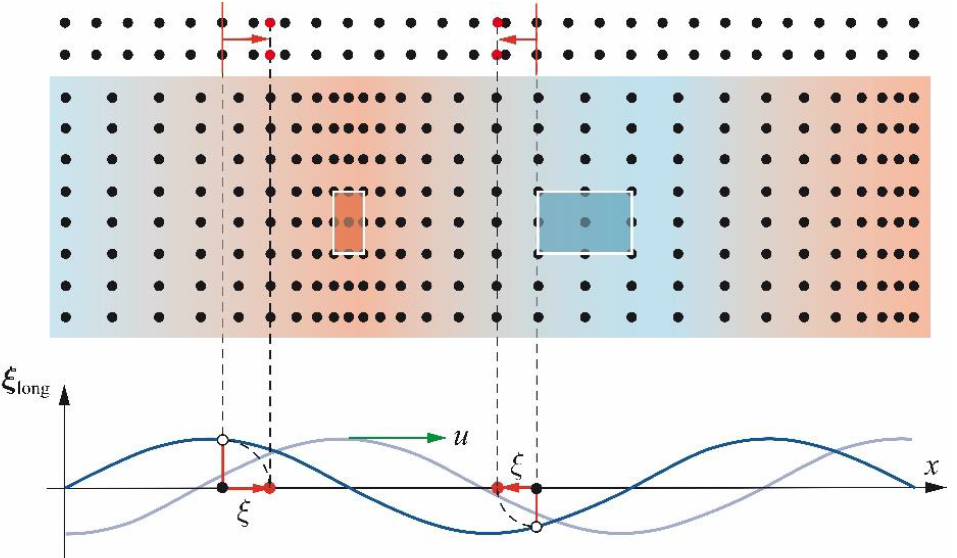
\includegraphics[height=2.6cm, align=t]{images/welle_longitudinal.png}
    \end{center}
    
    \textbf{Beispiel: } Schallwellen
\end{minipage}


\subsection[Wellengeschwindigkeit / Phasengeschwindigkeit]{Wellengeschwindigkeit / Phasengeschwindigkeit $\bm{u}$}

Die Störung an der Position $x_0$ zum Zeitpunkt $t=0$ breitet sich mit der Geschwindigkeit $u$ aus und erreicht nach einer Zeit $t$ die Position $x$

\begin{center}
    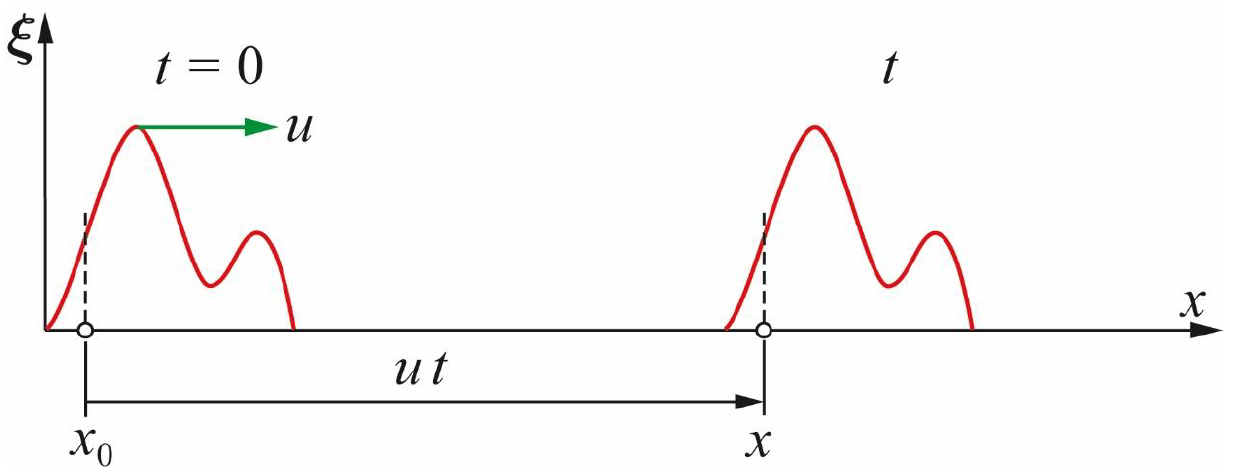
\includegraphics[width=0.62\columnwidth]{images/ausbreitung_stoerung.png}
\end{center}

\vspace{-0.4cm}

$$ \xi(x, t) = \xi(x - ut, 0) = f(x - ut) $$

\smallskip

\textbf{In einem Medium mit grösserer Dichte breiten sich Wellen schneller aus!} \\
\textrightarrow\ Bessere Kopplung der Moleküle

\smallskip

Man schaut bei der Beschreibung der Fortbewegung auf den Ort. Die Verschiebung des Ortes wird mit der Zeit hineingebracht.


\subsubsection{Verschiedene Wellengeschwindigkeiten}

\begin{minipage}{0.45\columnwidth}
    Schallwellen in Fluiden
\end{minipage}
\hfill
\begin{minipage}{0.48\columnwidth}
    $$\boxed{ u = \sqrt{\frac{1}{\rho \, \kappa}} }$$
\end{minipage}

\begin{minipage}{0.45\columnwidth}
    Schallwellen in Gasen
\end{minipage}
\hfill
\begin{minipage}{0.48\columnwidth}
    $$\boxed{ u = \sqrt{\frac{\varkappa \, p}{\rho}} = \sqrt{\frac{\varkappa \, R \, T}{M}} }$$
\end{minipage}

\begin{minipage}{0.45\columnwidth}
    Elastische Longitudinalwellen in einem schlanken Stab
\end{minipage}
\hfill
\begin{minipage}{0.48\columnwidth}
    $$\boxed{ u = \sqrt{\frac{E}{\rho}} }$$
\end{minipage}

\begin{minipage}{0.45\columnwidth}
    Elastische Transversalwellen
\end{minipage}
\hfill
\begin{minipage}{0.48\columnwidth}
    $$\boxed{ u = \sqrt{\frac{G}{\rho}} }$$
\end{minipage}

\begin{minipage}{0.45\columnwidth}
    Transversalwellen auf einem Seil oder einer Saite
\end{minipage}
\hfill
\begin{minipage}{0.48\columnwidth}
    $$\boxed{ u = \sqrt{\frac{F}{\rho \, A}} }$$ 
\end{minipage}

\begin{minipage}{0.45\columnwidth}
    Elektromagnetische Wellen (transversal) \\
    (z.B. Lichtwellen)
\end{minipage}
\hfill
\begin{minipage}{0.48\columnwidth}
    $$\boxed{ u = \frac{c}{n} }$$
\end{minipage}


\renewcommand{\arraystretch}{1.15}
\begin{ctabular}{c l c}
    $u$         & Wellengeschwindigkeit                                                 & $[u] = \frac{\meter}{\second}$                    \\
    $A$         & Querschnittsfläche                                                    & $[A] = \meter\squared$                            \\
    $E$         & Elastizitätsmodul                                                     & $[E] = \frac{\newton}{\meter\squared} = \pascal$  \\
    $F$         & Spannkraft des Seils / der Saite                                      & $[F] = \newton$                                   \\
    $G$         & Schubmodul                                                            & $[G] = \frac{\newton}{\meter\squared} = \pascal$  \\
    $M$         & Molmasse                                                              & $[M] = \frac{\kilogram}{\mole}$                   \\
    $p$         & Druck                                                                 & $[p] = \pascal$                                   \\
    $R$         & Universelle Gaskonstante: $R = 8.314 \mathrm{\frac{J}{mol \cdot K}}$  & $[R] = \mathrm{\frac{J}{mol \cdot K}} $           \\
    $T$         & \textbf{Absolut-}Temperatur                                           & $[T] = \mathrm{K}$                                \\
    $\kappa$    & Kompressibilität                                                      & $[\kappa] = \frac{1}{\pascal}$                    \\
    $\varkappa$ & Adiabatenexponent                                                     & $[\varkappa] = 1$                                 \\
    $\rho$      & Dichte                                                                & $[\rho] = \frac{\kilogram}{\meter\cubed}$         \\
    $n$         & Brechungsindex                                                        & $[n] = 1$                                         \\
    $c$         & Lichtgeschwindigkeit: $c = 300 \cdot 10^6 \, \frac{\meter}{\second}$  & $[c] = \frac{\meter}{\second}$
\end{ctabular}
\renewcommand{\arraystretch}{1}


\subsection{Wellengleichungen}

Die Wellengleichungen stellen eine \textbf{Verbindung zwischen Zeit und Ort} her.

\medskip
\begin{minipage}{0.45\columnwidth}
    Eindimensional \\
    Welle breitet sich in 1D aus
\end{minipage}
\hfill
\begin{minipage}{0.48\columnwidth}
    $$\boxed{ \frac{\partial^2 \xi}{\partial x^2} = \frac{1}{u^2} \frac{\partial^2 \xi}{\partial t^2}  }$$
\end{minipage}

\begin{minipage}{0.45\columnwidth}
    Zweidimensional \\
    Welle breitet sich in 2D aus
\end{minipage}
\hfill
\begin{minipage}{0.48\columnwidth}
    $$\boxed{ \frac{\partial^2 \xi}{\partial x^2} + \frac{\partial^2 \xi}{\partial y^2} = \frac{1}{u^2} \frac{\partial^2 \xi}{\partial t^2}  }$$
\end{minipage}

\begin{minipage}{0.45\columnwidth}
    Dreidimensional \\
    Welle breitet sich in 3D aus
\end{minipage}
\hfill
\begin{minipage}{0.48\columnwidth}
    $$\boxed{ \frac{\partial^2 \xi}{\partial x^2} + \frac{\partial^2 \xi}{\partial y^2} + \frac{\partial^2 \xi}{\partial z^2} = \frac{1}{u^2} \frac{\partial^2 \xi}{\partial t^2}  }$$
\end{minipage}


\subsubsection{Wichtige Lösung der Wellengleichung (1D)}

\begin{minipage}{0.38\columnwidth}
    $$\frac{\partial^2 \xi}{\partial x^2} = \frac{1}{u^2} \frac{\partial^2 \xi}{\partial t^2} $$
\end{minipage}
\hfill
\begin{minipage}{0.58\columnwidth}
    Ansatz: $\xi(x,t) = \xi_0 \cdot \sin(\omega \, t - k \, x)$
\end{minipage}

$$ \underbrace{- k^2 \, A \, \sin(\omega \, t - k \, x)}_{\substack{\frac{\partial^2 \xi}{\partial x^2} }} = - \frac{1}{u^2} \cdot \underbrace{ \omega^2 \, A \,\sin(\omega \, t - k \, x)}_{\substack{\frac{\partial^2 \xi}{\partial t^2} }}  $$ 

$$ \boxed{ \text{mit Lösung} \quad  u^2 = \frac{\omega^2}{k^2} } $$


\subsection{Harmonische Wellen}

$$ \boxed{ \xi(x, t) = \xi_0 \cdot \sin( \omega \, t - k \, x + \varphi) }  $$


\subsubsection{Terminologie}

\begin{center}
    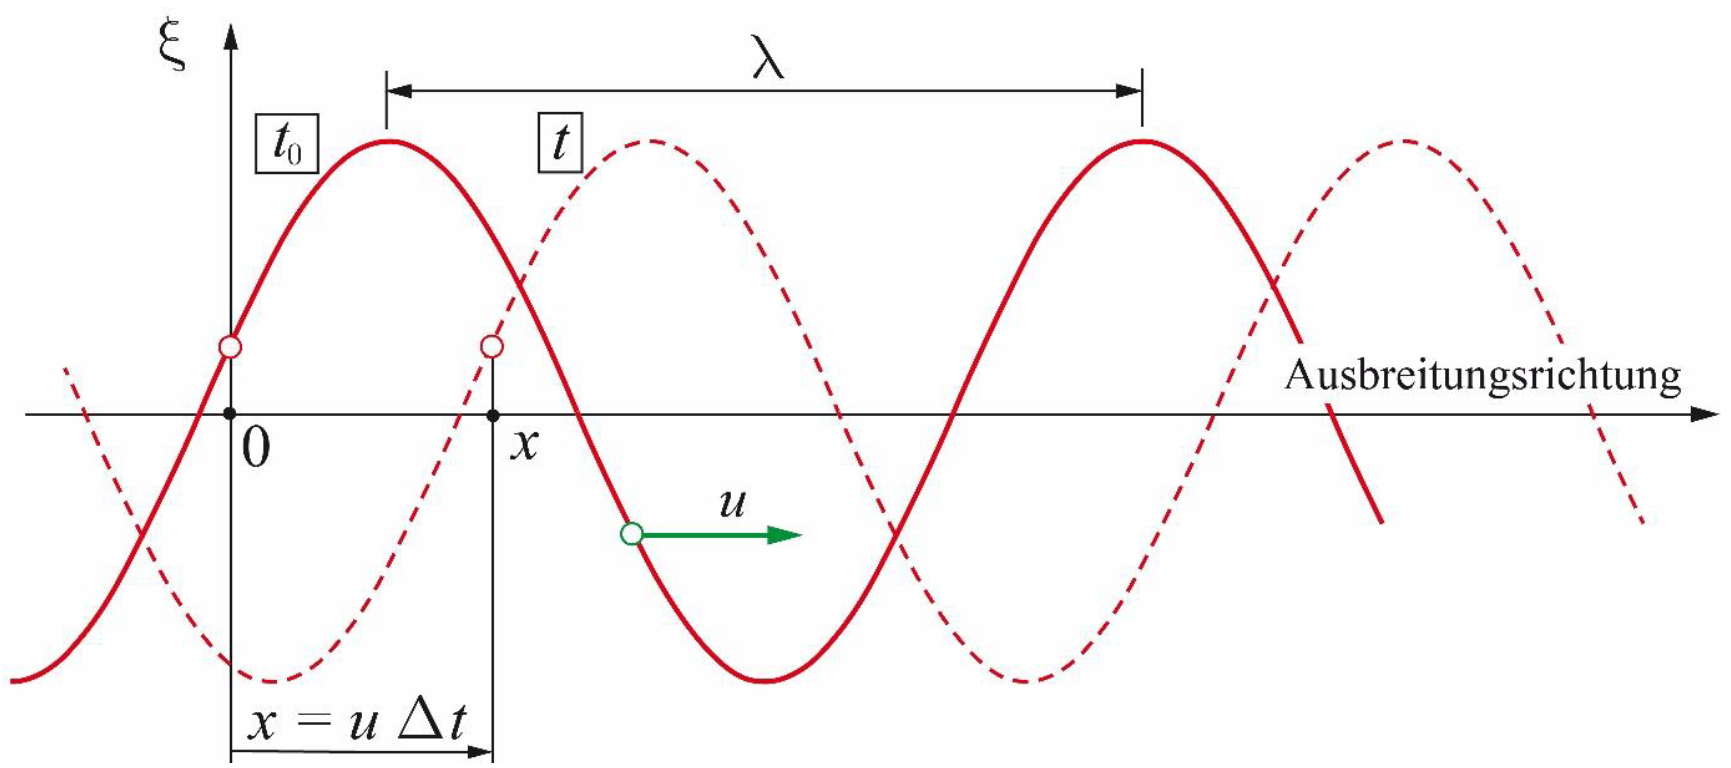
\includegraphics[width=0.7\columnwidth]{images/harmonische_wellen_terminologie.png}
\end{center}

\renewcommand{\arraystretch}{1.2}
\begin{ctabular}{c l c}
    $\xi_0$     & Amplitude             & $[\xi_0]$                         \\
    $\omega$    & Kreisfrequentz        & $[\omega] = \frac{\rad}{\second}$ \\
    $T$         & Periodendauer         & $[T] = \second$                   \\
    $k$         & Wellenzahl            & $[k] = \frac{1}{\meter}$          \\
    $\lambda$   & Wellenlänge           & $\lambda = \meter $               \\
    $u$         & Wellengeschwindigkeit & $[u] = \frac{\meter}{\second}$    \\
    $\varphi$   & Phasenverschiebung    & $[\varphi] = \rad$ 
\end{ctabular}
\renewcommand{\arraystretch}{1}


\subsubsection{Zusammenhänge}

\begin{center}
    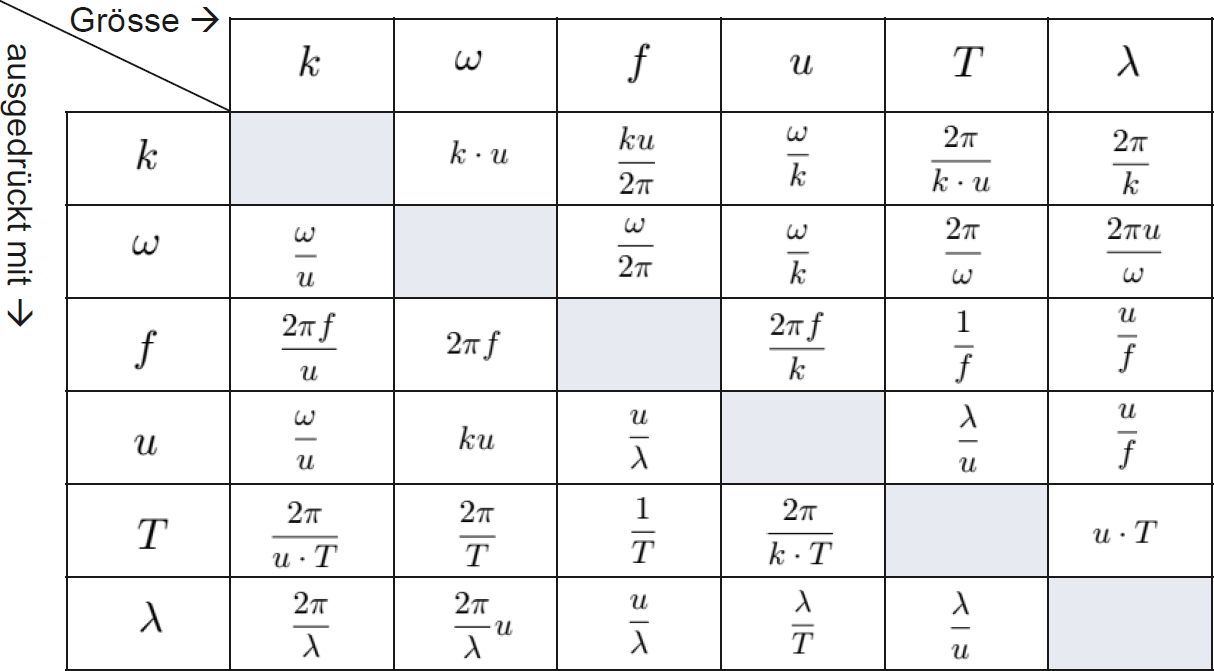
\includegraphics[width=0.9\columnwidth]{images/harmonische_wellen_zusammenhaenge.png}
\end{center}



\subsection{Wellenflächen / Wellenfronten}
Die Gesamtheit aller Punkte, die zu einer bestimmten Zeit im gleichen Schwingungszustand sind, bilden eine Fläche im Raum.

\smallskip

Diese \textbf{Flächen mit gleicher Phase} werden \textbf{Wellenflächen} oder \textbf{Wellenfronten} genannt.

\smallskip

Eine Welle kann sich in 3 Dimensionen ausbreiten und dabei \textbf{verschiedene Wellenflächen} zeigen. 


\subsection{Wellenausbreitung}

\begin{minipage}{0.25\columnwidth}
    Wellengleichung (3D)
\end{minipage}
\hfill
\begin{minipage}{0.73\columnwidth}
    $$\boxed{ \frac{\partial^2 \xi}{\partial x^2} + \frac{\partial^2 \xi}{\partial y^2} + \frac{\partial^2 \xi}{\partial z^2} = \frac{1}{u^2} \frac{\partial^2 \xi}{\partial t^2}  }$$
\end{minipage}

\begin{minipage}{0.25\columnwidth}
    Lösungsansatz
\end{minipage}
\hfill
\begin{minipage}{0.73\columnwidth}
    $$ \boxed{ \xi = \xi_0 e^{\jimg \, (\omega \, t - \vec{k} \bullet \vec{r})} }$$
\end{minipage}

\medskip

mit Wellenvektor $\vec{k} = \begin{pmatrix} k_x \\ k_y \\ k_z  \end{pmatrix}$ und Ortsvektor $ \vec{r} = \begin{pmatrix} r_x \\ r_y \\ r_z  \end{pmatrix}$


\subsubsection{Ebene Wellen}

\begin{minipage}[t]{0.3\columnwidth}
    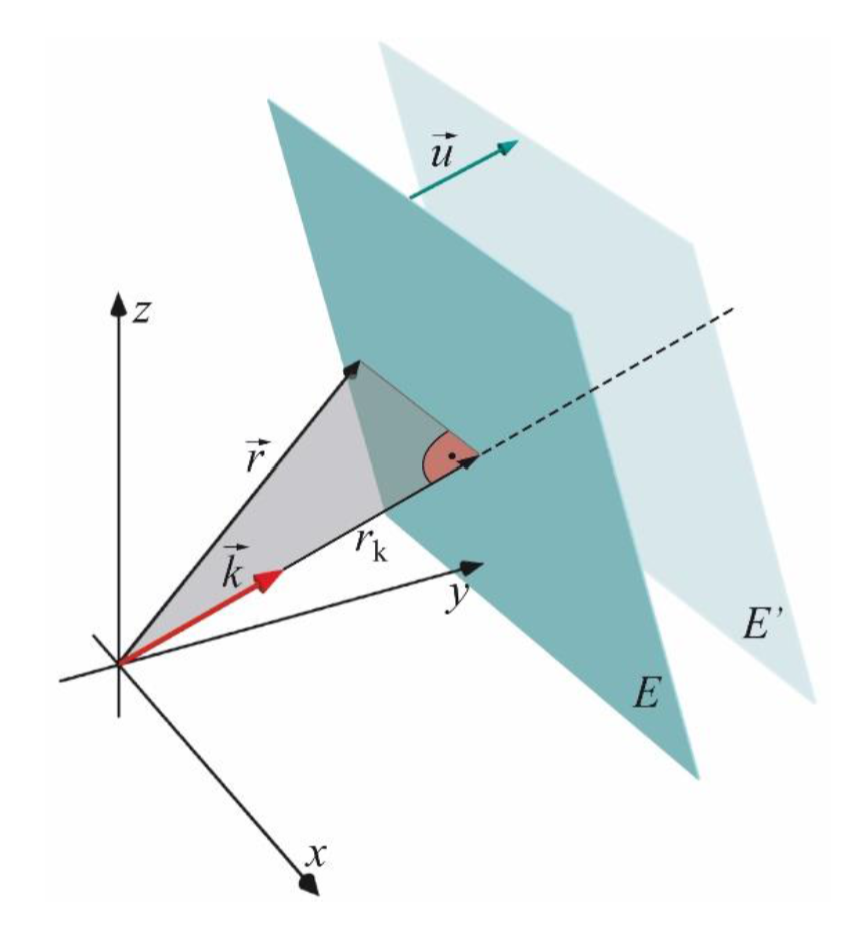
\includegraphics[width=\columnwidth, align=t]{images/Ebene_Welle.png}
\end{minipage}
\hfill
\begin{minipage}[t]{0.68\columnwidth}
    \begin{itemize}
        \item Wellenfronten sind Ebenen im Raum 
        \item Wellenvektor $\vec{k}$ steht senkrecht auf der Ebenen 
        \item \textbf{Abstand} zw. zwei Wellenfronten ist $\lambda$ 
    \end{itemize}

    \medskip

    Die Ebenen bewegen sich mit der Wellengeschwindigkeit
    $$ \boxed{ u = \frac{\omega}{k} \quad \text{ mit } k = ||\vec{k}|| = \sqrt{k_x^2 + k_y^2 + k_z^2} }$$  
    in die \textbf{Richtung}, die durch den \textbf{Wellenvektor} $\vec{k}$ gegeben ist.
\end{minipage}


\subsubsection{Kugelwellen}

\begin{minipage}[t]{0.3\columnwidth}
    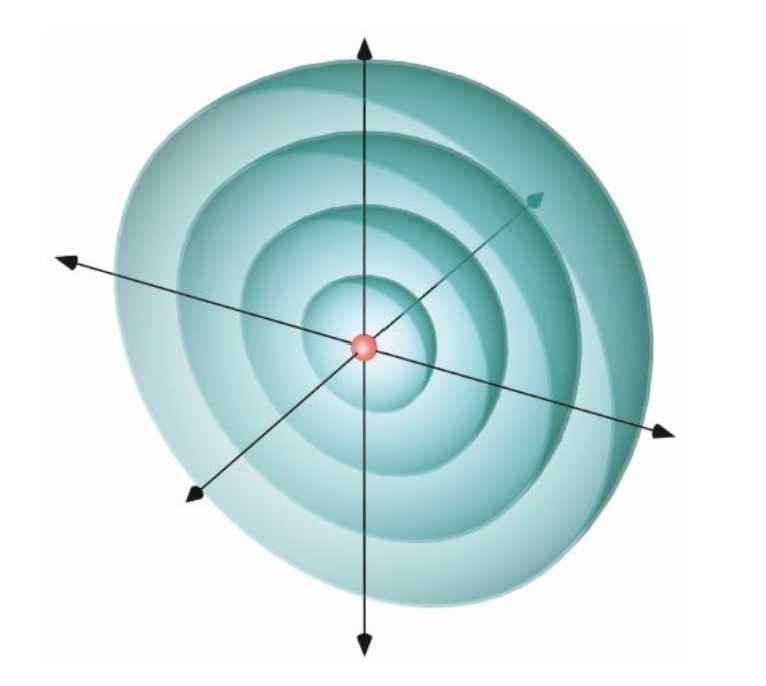
\includegraphics[width=\columnwidth, align=t]{images/Kugel_Welle.png}
\end{minipage}
\hfill
\begin{minipage}[t]{0.68\columnwidth}
    \begin{itemize}
        \item Wellenfronten sind Kugeln 
        \item Wellenvektor $\vec{k}$ steht senkrecht auf Wellenfronten 
        \item Wellenfronten bewegen sich mit der  Wellengeschwindigkeit vom Zentrum weg 
        \item Amplitude nimmt mit $\frac{1}{r}$ ab
    \end{itemize}
\end{minipage}

Für eine \textbf{punktförmige Quelle} und \textbf{keine Winkelabhängigkeit} gilt:

$$ \boxed{ \text{Wellengleichung:} \quad \frac{1}{u^2} \frac{\partial^2 \xi}{\partial t^2} = \frac{2}{r} \left( \frac{\partial \xi}{\partial r} \right) + \frac{\partial^2 \xi}{\partial r^2} }$$

$$ \boxed{ \text{Lösungsansatz:} \quad \xi(t, r) = \frac{1}{r} \xi_0 \, e^{ \jimg \, (\omega \, t - k \, r)} }  $$



\subsection{Bewegte Quellen}

\begin{minipage}[t]{0.46\columnwidth}
    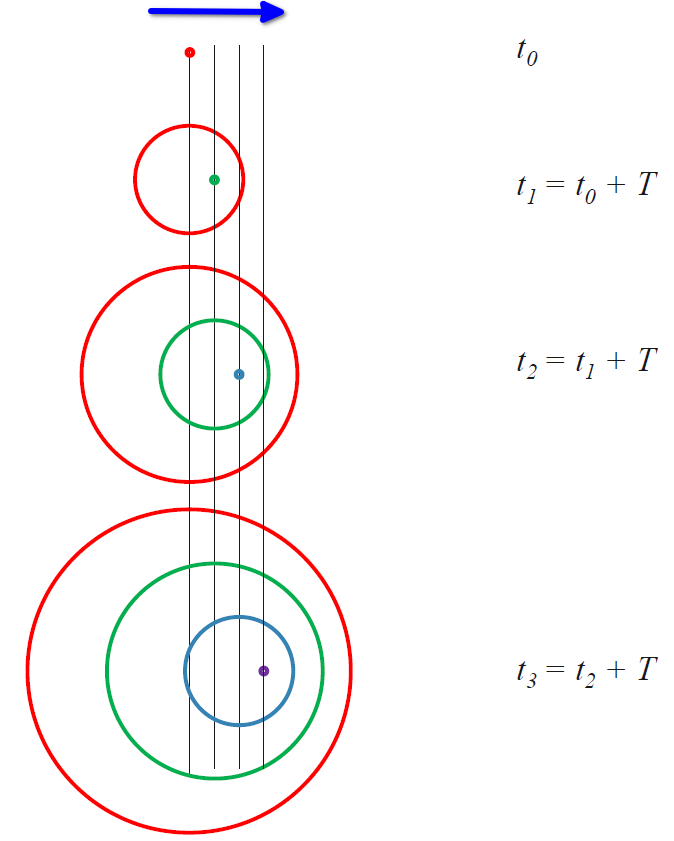
\includegraphics[width=\columnwidth, align=t]{images/Bewegte_Quellen.png}
\end{minipage}
\hfill
\begin{minipage}[t]{0.48\columnwidth}
    Die Quelle bewegt sich mit der \cbl{Geschwindigkeit $v_Q$} in eingezeichneter Richtung fort

    \medskip

    Die Quelle verschiebt sich in der Zeit $T$ um 
    $$ \boxed{ \Delta x = v_Q \cdot T }$$
\end{minipage}


\subsubsection{Frequenzverschiebung durch Bewegung der Quelle}


\begin{minipage}[t]{0.54\columnwidth}
    Die Quelle sendet eine Frequenz $f$ aus.
    Durch die Bewegung der Quelle ändert sich die Wellenlänge $\lambda$ und somit ergibt sich eine neue Frequenz $f'$, welche ein statischer Beobachter wahrnimmt.
    
    \vspace{-0.2cm}

    $$ \boxed{f' = \frac{1}{ \left( 1 \mp \frac{v_Q}{u} \right)}f} $$

    \begin{tabular}{@{}ll@{}}
        $+$ & Quelle bewegt sich vom Beobachter weg \\
        $-$ & Quelle bewegt sich zum Beobachter hin
    \end{tabular}
\end{minipage}
\hfill
\begin{minipage}[t]{0.42\columnwidth}
    \paragraph{Herleitung}

    \vspace{-0.5cm}

    \begin{align*}
        \lambda'    &= \lambda -v_Q \cdot T                         \\
        \lambda'    &= \lambda -v_Q \frac{\lambda}{u}               \\
        \lambda'    &= \lambda \left( 1 - \frac{v_Q}{u} \right)     \\
        f'          &= \frac{u}{\lambda'} = \frac{u}{\lambda \left( 1-\frac{v_Q}{u} \right)} = \frac{f}{ \left( 1-\frac{v_Q}{u} \right)}
    \end{align*}
\end{minipage}


\renewcommand{\arraystretch}{1.2}
\begin{ctabular}{clc}
    $\lambda$   & Wellenlänge der aussendeten Welle     & $[\lambda] = \meter$              \\
    $\lambda'$  & Wellenlänge der wahrgenommenen Welle  & $[\lambda'] = \meter$             \\
    $v_Q$       & Geschwindigkeit der bewegten Quelle   & $[v_Q] = \frac{\meter}{\second}$  \\
    $u$         & Wellengeschwindigkeit                 & $[u] = \frac{\meter}{\second}$    \\
    $f$         & Frequenz der ausgesendeten Wellen     & $[f] = \hertz$                    \\
    $f'$        & Frequenz der wahrgenommenen Wellen    & $[f'] = \hertz$                   \\
    $T$         & Periodendauer (Dauer der Ausbreitung) & $[T] = \second$
\end{ctabular}
\renewcommand{\arraystretch}{1}


\subsubsection{Bewegte Quelle vs. unbewegte Quelle}

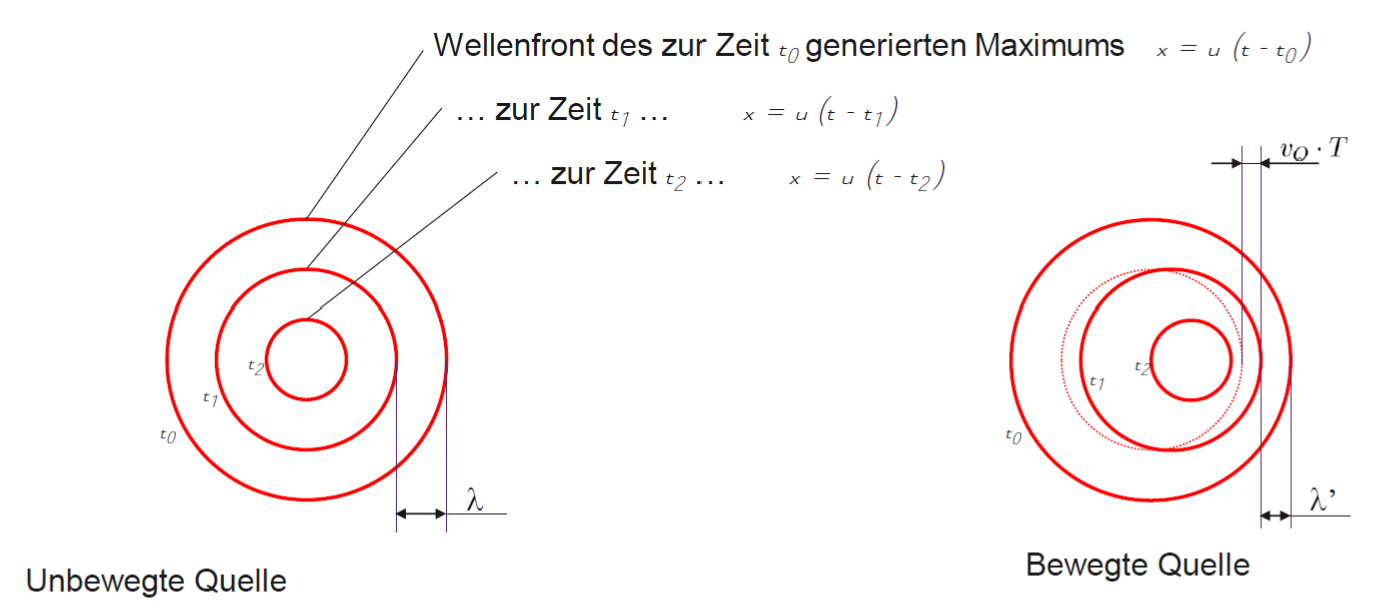
\includegraphics[width=\columnwidth]{images/Unbewegte_Quelle.png}


\subsection{Doppler Effekt}
Die \textbf{Veränderung der Wellenlänge} $\lambda$ der von einer \textbf{bewegten Quelle} ausgesandten Wellen ist als \textbf{Doppler Effekt} bekannt.

\begin{center}
    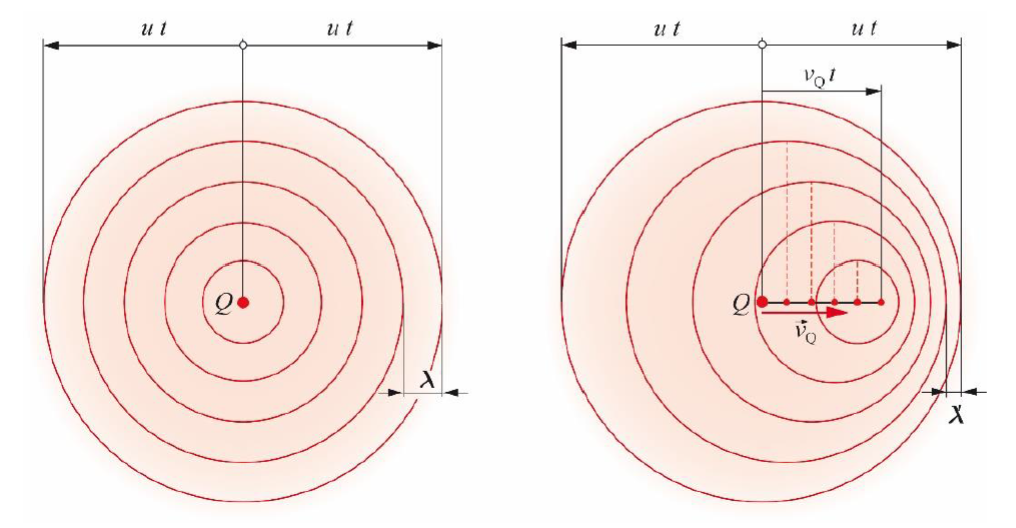
\includegraphics[width=0.8\columnwidth]{images/Doppler_effekt.png}
\end{center}


\subsection{Bewegte Quelle mit Winkel}
Die Quelle bewegt sich nicht direkt auf den Beobachter zu, sondern sie bewegt sich am \textbf{Beobachter vorbei}

\begin{minipage}{0.48\columnwidth}
    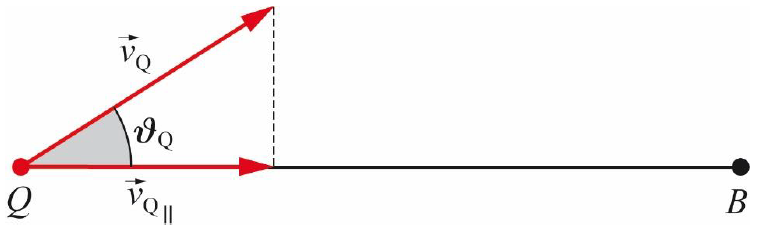
\includegraphics[width=\columnwidth]{images/bewegte_quelle_winkel.png} 
\end{minipage}
\hfill
\begin{minipage}{0.48\columnwidth}
    $$ \boxed{ f' =  \frac{1}{1 - \frac{v_Q}{u} \cdot \cos(v_Q)}  \, f} $$
\end{minipage}

\begin{ctabular}{clc}
    $v_Q$   & Geschwindigkeit der bewegten Quelle   & $[v_Q] = \frac{\meter}{\second}$  \\
    $u$     & Wellengeschwindigkeit                 & $[u] = \frac{\meter}{\second}$    \\
    $f$     & Frequenz der ausgesendeten Wellen     & $[f] = \hertz$                    \\
    $f'$    & Frequenz der wahrgenommenen Wellen    & $[f'] = \hertz$
\end{ctabular}


\subsubsection{Beispiel Winkel zw. Quelle und Beobachter}

\begin{minipage}[t]{0.4\columnwidth}
    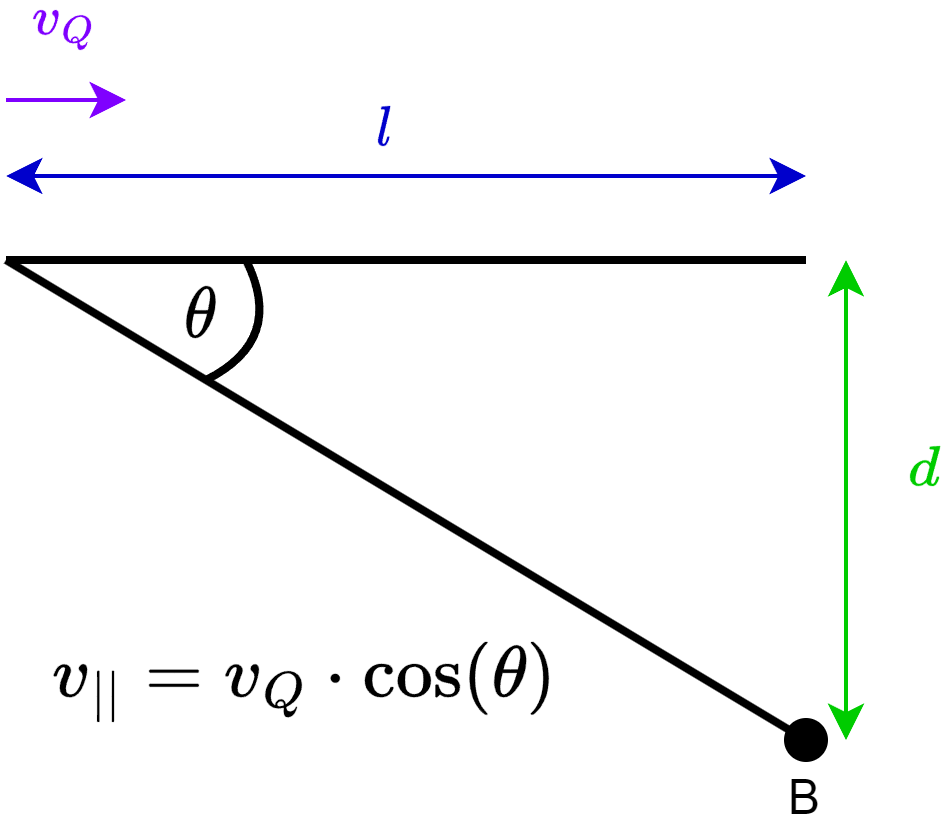
\includegraphics[width=\columnwidth, align=t]{images/beispiel_bewegte_quelle.png} 
\end{minipage}
\hfill
\begin{minipage}[t]{0.58\columnwidth}
    \textbf{Gegeben:} $v_Q, \, \theta, \,u, \,d, \,l$ \qquad 
    \textbf{Gesucht:} $\frac{f'}{f}$
    $$f' =  \frac{1}{1 - \frac{v_Q}{u} \cdot \cos(v_Q)}$$
    \[
        \tan(\theta) = \frac{d}{l} =  \frac{\sin(\theta)}{\cos(\theta)} \qquad
        \sin^2(\theta) = 1 - \cos^2(\theta)
    \]

    $$ \Rightarrow\ \tan(\theta) = \frac{d}{l} = \frac{\sqrt{ 1 - \cos^2(\theta)}}{\cos(\theta)} $$

    \[
        \frac{1}{\cos^2(\theta)} = \frac{d^2}{l^2} + 1  \qquad
        \cos^2(\theta) = \frac{1}{1 + \frac{d^2}{l^2}}
    \]
\end{minipage}

$$ \boxed{ \Rightarrow\ \frac{f'}{f} = \frac{1}{1 - \frac{v_Q}{u} \cdot \sqrt{\frac{l^2}{l^2 + d^2} } } } $$


\subsection{Bewegter Beobachter}

\begin{minipage}[l]{0.48\columnwidth}
    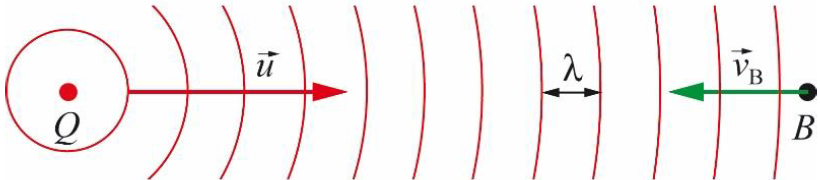
\includegraphics[width=\columnwidth, align=t]{images/bewegter_beobachter.png}
    \end{minipage}
\hfill
\begin{minipage}[l]{0.48\columnwidth}
    $$ \boxed{f' = \left( 1 \pm \frac{v_B}{u}  \right) \, f } $$

    \begin{tabular}{ll}
        $+$ & Beobachter geht auf Quelle zu \\
        $-$ & Beobachter geht von Quelle weg
    \end{tabular}
\end{minipage}


\renewcommand{\arraystretch}{1.2}
\begin{ctabular}{clc}
    $v_B$   & Geschwindigkeit des bewegten Beobachters  & $[v_B] = \frac{\meter}{\second}$  \\
    $v_Q$   & Geschwindigkeit der bewegten Quelle       & $[v_Q] = \frac{\meter}{\second}$  \\
    $u$     & Wellengeschwindigkeit                     & $[u] = \frac{\meter}{\second}$    \\
    $f_B$   & Frequenz, welche Beobachter wahrnimmt     & $[f_B] = \hertz$                  \\
    $f_Q$   & Frequenz, welche Quelle 'aussendet'       & $[f_Q] = \hertz$ 
\end{ctabular}
\renewcommand{\arraystretch}{1}



\subsection{Bewegte Quelle und bewegter Beobachter}

\begin{minipage}[c]{0.48\columnwidth}
    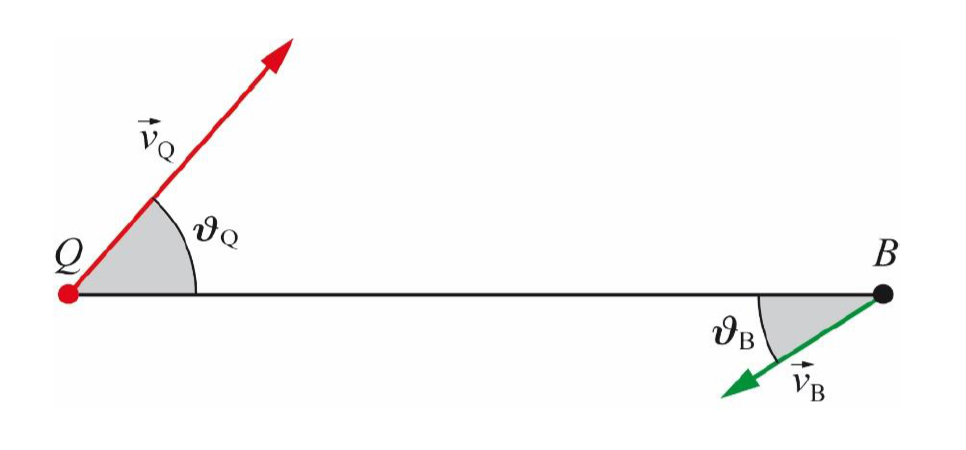
\includegraphics[width=\columnwidth]{images/akustischer_doppler_effekt.png} 
\end{minipage}
\hfill
\begin{minipage}[c]{0.48\columnwidth}
    $$ \boxed{f_B = \frac{u+ v_B \cos(\vartheta_B)}{u- v_Q \cos(\vartheta_Q)}f_Q} $$
\end{minipage}

\renewcommand{\arraystretch}{1.2}
\begin{ctabular}{clc}
    $\vartheta_B = \theta_B$    & siehe Skizze                          & $[\vartheta_B] = \degree$         \\
    $v_B$                       & Geschwindigkeit bewegter Beobachter   & $[v_B] = \frac{\meter}{\second}$  \\
    $\vartheta_Q = \theta_Q$    & siehe Skizze                          & $[\vartheta_Q] = \degree$         \\
    $v_Q$                       & Geschwindigkeit bewegte Quelle        & $[v_Q] = \frac{\meter}{\second}$  \\
    $u$                         & Wellengeschwindigkeit                 & $[u] = \frac{\meter}{\second}$    \\
    $f_B$                       & Frequenz beim bewegten Beobachter     & $[f_B] = \hertz$                  \\
    $f_Q$                       & Frequenz bei der bewegten Quelle      & $[f_Q] = \hertz$
\end{ctabular}
\renewcommand{\arraystretch}{1}


\subsubsection{Optischer Doppler Effekt}

\textbf{Wird verwendet, wenn die Wellengeschwindigkeit $\boldsymbol{u}$ gleich der Lichtgeschwindigkeit $\boldsymbol{c}$ ist!}

Es spielt nur die \textbf{relative} Bewegung von Beobachter und Quellen eine Rolle

$$ \boxed{f' = \frac{\sqrt{1-\beta^2}}{1 - \beta \cos(\vartheta)}f \qquad  \text{ mit} \quad \beta = \frac{v}{c} } $$

\vspace{-0.2cm}

\begin{align*}
    \text{für } \beta \ll 1 \qquad f'                                            &\simeq \frac{1}{1- \beta \cdot \cos(\theta)} \cdot f \\
    \text{für } \beta \ll 1 \text{ und } \theta \approx \frac{\pi}{2} \qquad f'  &\simeq \frac{1}{1- \beta } \cdot f
\end{align*}



\subsubsection{Mach'scher Kegel}

Wenn sich die Quelle schneller fortbewegt als die Wellengeschwindigkeit, dann entsteht ein Mach'scher Kegel

\begin{minipage}[t]{0.6\columnwidth}
    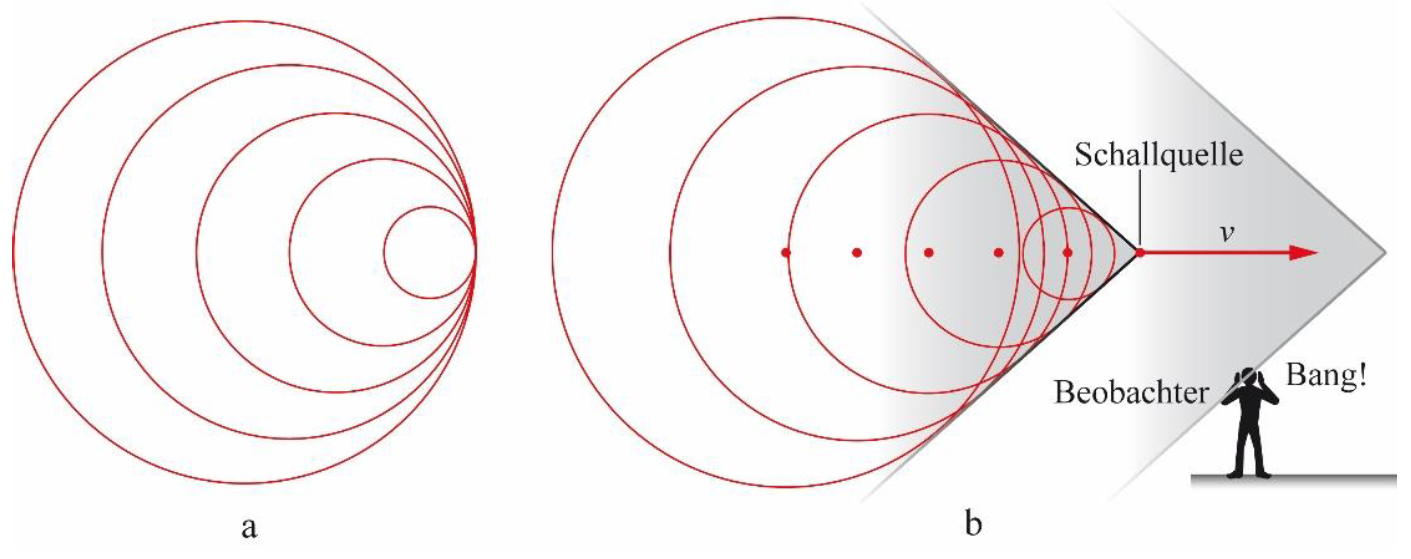
\includegraphics[height=2.2cm, align=t]{images/machkegel_1.png} 
    $$ \boxed{ \sin(\vartheta) = \frac{u \, \Delta t}{v \, \Delta t} = \frac{u}{v} } $$
\end{minipage}
\hfill
\begin{minipage}[t]{0.38\columnwidth}
    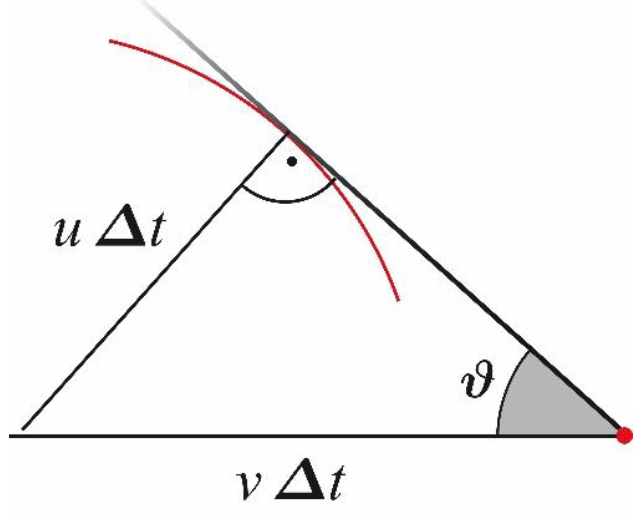
\includegraphics[height=2.2cm, align=t]{images/machkegel_2.png} 
    $$ \boxed{ M = \frac{v}{u} } $$
\end{minipage}


\renewcommand{\arraystretch}{1.1}
\begin{ctabular}{clc}
    $v$ & Geschwindigkeit der Quelle                        & $[v] = \frac{\meter}{\second}$    \\
    $u$ & Wellengeschwindigkeit (Schallgeschwindingkeit)    & $[u] = \frac{\meter}{\second}$    \\
    $M$ & Machzahl                                          & $[M] = 1$
\end{ctabular}
\renewcommand{\arraystretch}{1}


\subsection{Wellenwiderstand, Energietransport -- Schallwellen}

\subsubsection{Terminologie Wellenwiderstand}
Der \textbf{Wellenwiderstand $Z$} (auch \textbf{Impedanz} genannt) beschreibt, wie ein Medium den Fluss von Energie beeinflusst.

\smallskip

\textrightarrow\ \textquotesingle Wie gut können sich Wellen in einem Medium ausbreiten?\textquotesingle

$$ \boxed{ Z = \rho \cdot u = \frac{\Delta p_0}{v_0} } $$


\renewcommand{\arraystretch}{1.4}
\begin{ctabular}{clc}
    $Z$             & Wellenwiderstand bzw. Impedanz    & $[Z] = \ohm = \frac{\pascal}{\meter\per\second} = \frac{\newton \, \second}{\meter\cubed}$    \\
    $\rho$          & Dichte des Mediums                & $[\rho] = \frac{\kilogram}{\meter\cubed}$                                                     \\
    $u$             & Wellengeschwindigkeit             & $[u] = \frac{\meter}{\second}$                                                                \\
    $\Delta p_0$    & Druckamplitude                    & $[\Delta p_0] = \pascal$                                                                      \\
    $v_0$           & Schnellenamplitude                & $[v_0] = \frac{\meter}{\second}$
\end{ctabular}
\renewcommand{\arraystretch}{1}


\subsubsection{Weitere Terminologien}

\renewcommand{\arraystretch}{1.2}
\begin{tabular}{lll}
    Schalldruck                 & $p = \Delta p_0 \, \cos(\omega \, t - k \, x)$    & $[p] = \pascal$                   \\
    Druckamplitude              & $  \Delta p_0 = \rho \, u \, v_0 $                &                                   \\
    \\
    Schallschnelle (Schnelle)   & $v = v_0 \,  \cos(\omega \, t - k \, x)$          & $[v] = \frac{\meter}{\second}$    \\
    Schnellenamplitude          & $v_0 = \omega \, \xi_0$ 
\end{tabular}
\renewcommand{\arraystretch}{1}


\subsubsection{Intensität der Schallwelle}

\textbf{Intensität = gemittelte Energieflussdichte}

\begin{minipage}{0.48\columnwidth}
    $$ E_{\rm kin} = \frac{\rho \cdot v^2}{4} = \frac{\rho \cdot v_0^2}{4} $$
\end{minipage}
\hfill
\begin{minipage}{0.48\columnwidth}
    $$ E_{\rm pot} = \frac{p^2 - p_0^2}{2 \, \rho \, u^2} = \frac{\rho \cdot v_0^2}{4} $$
\end{minipage}

$$ E_{\rm tot} = E_{\rm kin} + E_{\rm pot} = \frac{\rho \cdot v_0^2}{2} $$

$$ \boxed{ I = u \cdot \overline{w} = \frac{1}{2} \rho \, v_0^2 \, u  =  \frac{1}{2} \rho \, (\omega \, \xi_0)^2  \, u = \frac{( \Delta p_0)^2}{2 \, Z} = \frac{P}{A} } $$


\renewcommand{\arraystretch}{1.2}
\begin{ctabular}{clc}
    $I$             &  Schallintensität                                 & $[I] = \frac{\watt}{\meter\squared}$                                                          \\
    $\overline{w}$  & Energieflussdichte                                & $[\overline{w}] = \frac{\watt \, \second}{\meter\cubed}$                                      \\
                    & Pot. Energie \textrightarrow\ 'Kompression Gas'   &                                                                                               \\
                    & Kin. Energie \textrightarrow\ 'Geschw. Teilchen'  &                                                                                               \\
    $\rho$          & Dichte                                            & $[\rho] = \frac{\kilogram}{\meter\cubed}$                                                     \\
    $v_0$ &         Schnellenamplitude                                  & $[v_0] = \frac{\meter}{\second}$                                                              \\
    $\xi_0$         & Amplitude                                         & $[\xi_0]$                                                                                     \\
    $u$             & Wellengeschwindigkeit                             & $[u] = \frac{\meter}{\second}$                                                                \\
    $\Delta p_0$    & Druckamplitude                                    & $[\Delta p_0] = \pascal$                                                                      \\
    $Z$             & Wellenwiderstand bzw. Impedanz                    & $[Z] = \ohm = \frac{\pascal}{\meter\per\second} = \frac{\newton \, \second}{\meter\cubed}$    \\
    $P$             & Leistung                                          & $[P] = \watt$                                                                                 \\
    $A$             & (Abstrahl-) Fläche                                & $[A] = \meter\squared$ 
\end{ctabular}
\renewcommand{\arraystretch}{1}


\subsection{Dispersion}
Die \textbf{Abhängigkeit} der Wellengeschwindigkeit \textbf{von der Wellenlänge} wird als Dispersion bezeichnet.

\smallskip

\textrightarrow\  Siehe Beispiel Optik Abschnitt~\ref{Dispersion Optik}


\subsubsection{Dispersion bei Wasserwellen}

$$ \boxed{ u(\lambda) = \sqrt{\left( \frac{g \cdot \lambda}{2 \, \pi} + \frac{2 \, \pi \cdot \sigma}{\rho \cdot \lambda} \right) \cdot \tanh \left( \frac{2 \, \pi \cdot h}{\lambda} \right) }  } $$


\begin{minipage}{0.48\columnwidth}
    \begin{center}
        Tiefes Wasser ($\lambda \ll h$)
    \end{center}
    $$ \boxed{ u(\lambda) = \sqrt{\frac{g \cdot \lambda}{2 \, \pi}} } $$
\end{minipage}
\hfill
\begin{minipage}{0.48\columnwidth}
    \begin{center}
        Flaches Wasser ($\lambda \gg h$)
    \end{center}
    $$ \boxed{ u = \sqrt{ g \cdot h } } $$
\end{minipage}


\renewcommand{\arraystretch}{1.2}
\begin{ctabular}{clc}
    $g$         & Erdbeschleinigung $g = 9.81 \, \frac{\meter}{\second\squared}$    & $[g] = \frac{\meter}{\second\squared}$    \\
    $\lambda$   & Wellenlänge                                                       & $[\lambda] = \meter $                     \\
    $\sigma$    & Oberflächenspannung                                               & $[\sigma] = \frac{\newton}{\meter}$       \\
    $h$         & Wassertiefe                                                       & $[h] = \meter$                            \\
    $\rho$      & Dichte                                                            & $[\rho] = \frac{\kilogram}{\meter\cubed}$
\end{ctabular}
\renewcommand{\arraystretch}{1}

